\section{The Summer Expedition Student Prospectus}

\textbf{Dates}: 12th July -> 17th August 2008 (5 weeks)

\tweet{3:54PM Jul 19, 2008}{Belgium. Andy driving. Trance. Sunny. Three lanes. Van air a bit thick already. Shadows of rooftop barrels cast on tarmac.}

\textbf{Logistiscs}: We'll be taking the usual heavily-overladen 9-seater
minibus via the autobahn (1000miles), with spaces reserved for
Drivers and the Poor (undergrads). Everyone else to fly.
Base camp (where we park the bus) is at Ravne at 912m, the
Bivvi (mountain camp) is at 1850m or so: and all the cheese,
equipment, tents \& etc. needs to be carried up on our backs!

\subsection{Why on Earth would I want to do this?}

Many reasons! This is your opportunity to find something BIG, have an absolutely cracking summer a world away from \passage[town]{London} living in the wild battling with the rock and the storms above. If you've got any hunger for adventure, or a thirst to be first – you will not want to miss out on this.

Living on top of a mountain drinking snow melt is great fun (if at little stone-age sometimes), and we'll be
caving with the JSPDT. Eastern Europe's amazing and completely different to elsewhere – don't faff around
interrailing visiting Tourist traps, come and visit a country properly and learn the Slovene for “Cheese, Please, Yes, Please, Cheese!”

Also, you'd be joining in a very exciting year – the oft hypothesised connection between the two systems in almost unbearably close now, and you will have a serious chance of being there both at the big moment, and to bask in the glory afterwards!

\begin{pagefigure}
\checkoddpage \ifoddpage \forcerectofloat \else \forceversofloat \fi
\centering
\frame{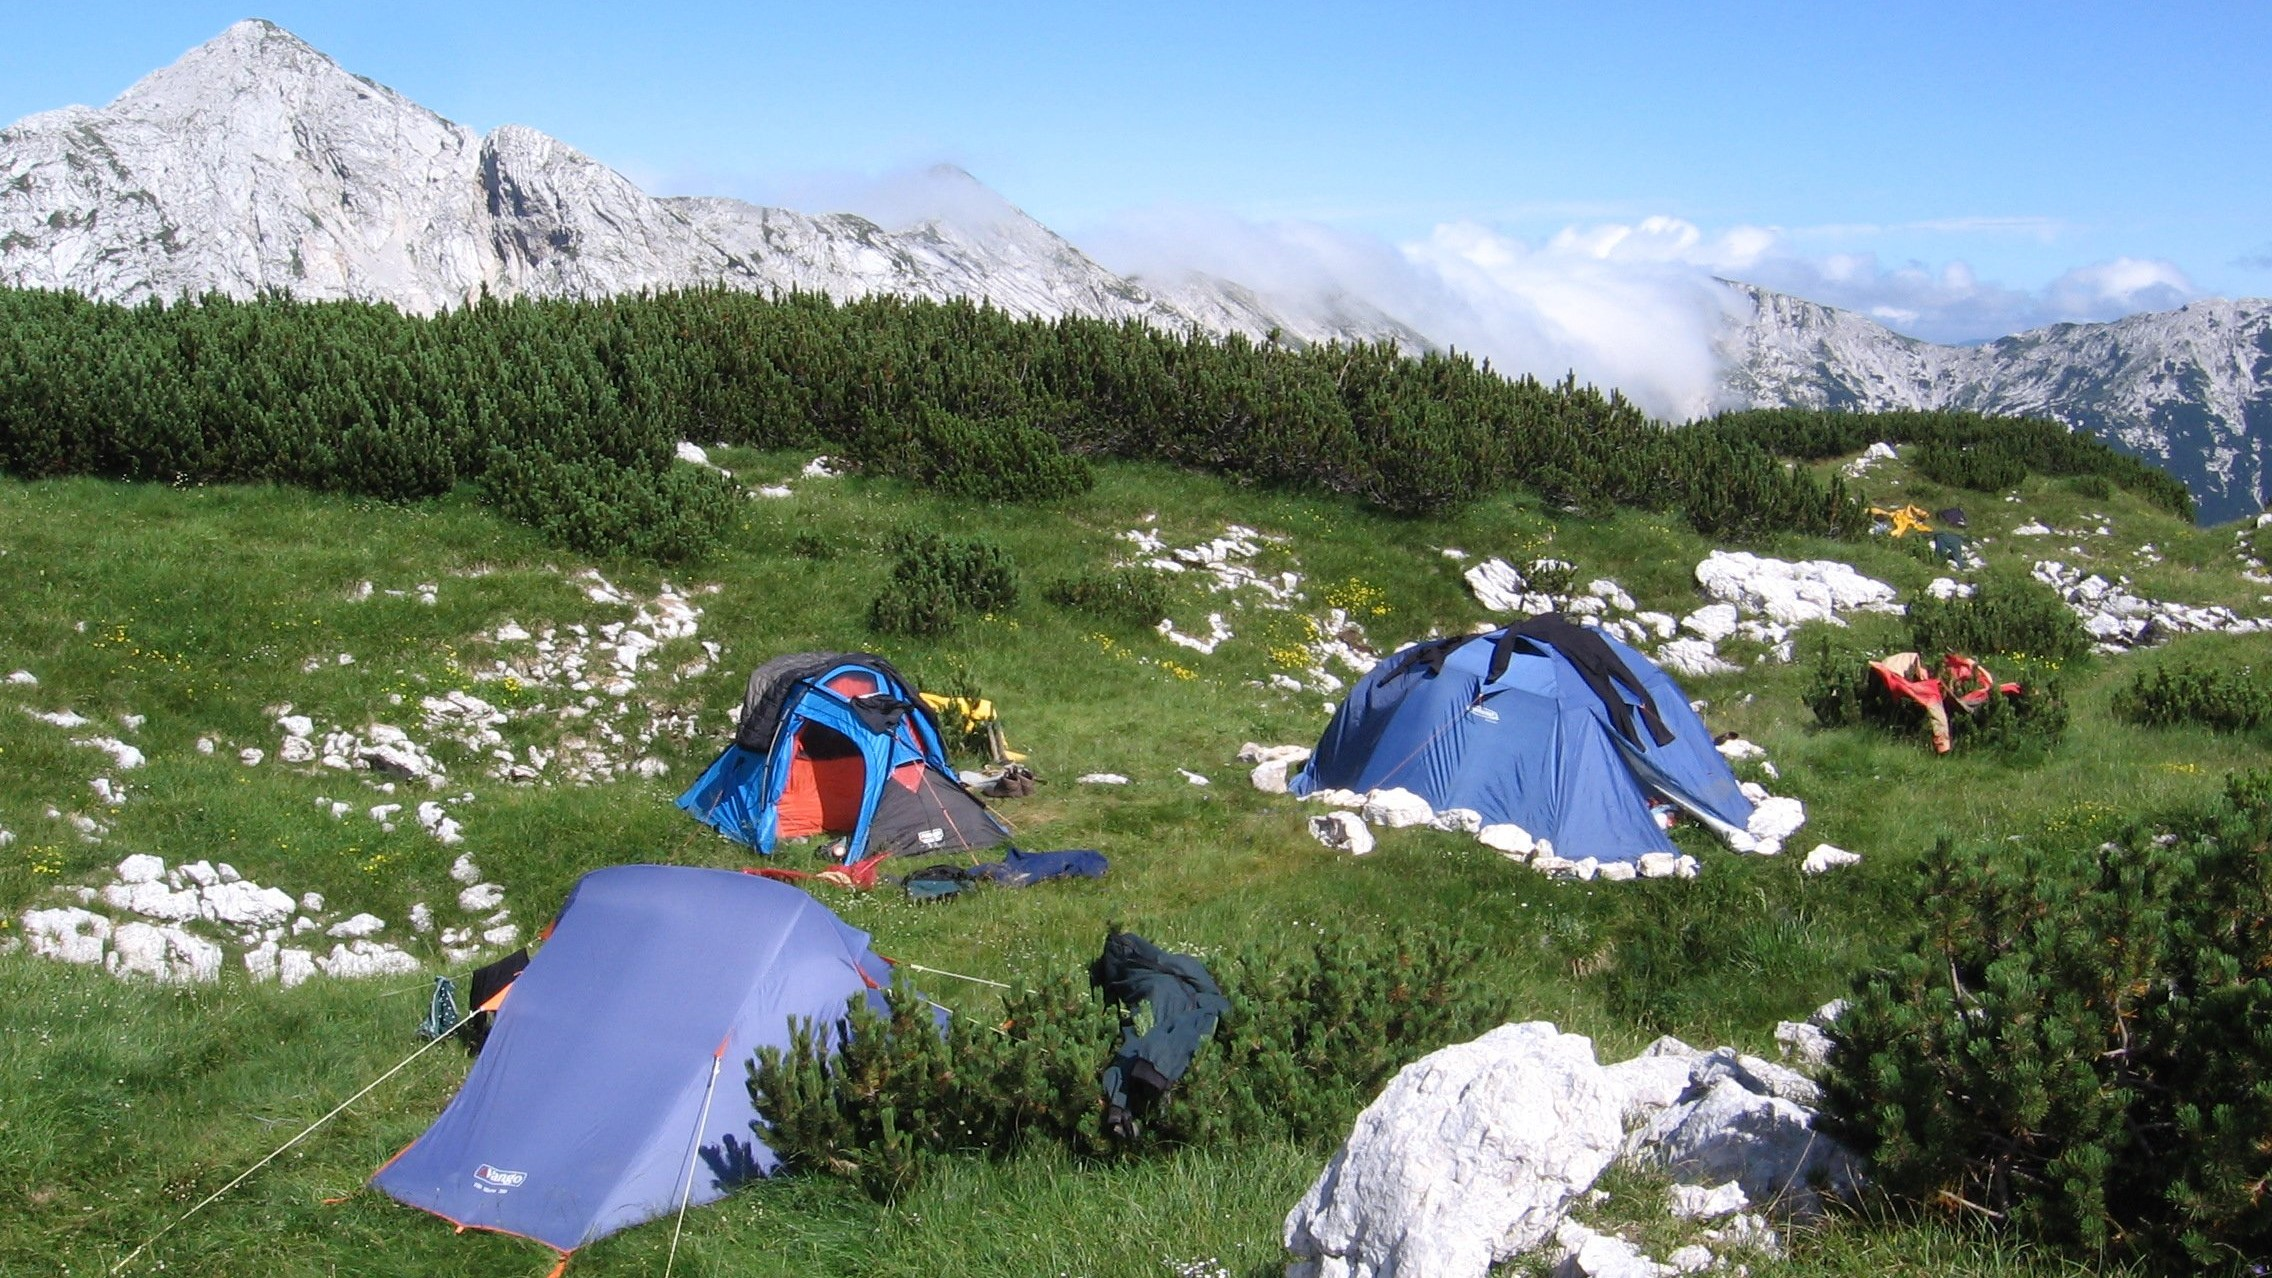
\includegraphics[width=\textwidth]{2008/why/Jarvist Frost - canon a520 - tents on plateau2--orig.jpg}}
\caption{A beautiful day on the \passage{Migovec plateau}. \pic{Jarvist Frost}} \label{tents}
\end{pagefigure}